\documentclass[font=default]{mpltx}
\usepackage{bm, ctex, array}
\usepackage{subfigure, graphicx}
\usepackage{multirow}
% 以下至 \begin{document} 都仅是本文件为了方便额外定义的命令, 写报告时不需要.
\hypersetup{colorlinks=false}% 超链接带颜色
\usepackage{xcolor}
% 以上是本文件为了方便额外定义的命令, 写报告时不需要.
\linespread{1.5}
\begin{document}

\title{扫描电子显微镜} % 切合报告内容, 简短明确, 可以不同于讲义
\author{MaskedName} % 这里 \emailphone 一定要紧跟在 \author 后方
\emailphone{MyMail@stu.pku.edu.cn}{Tel}
% 如果改用 \email 则仅需要邮箱参数
\affiliation{北京大学物理学院\quad 学号: StudentID}
\date{\zhdate{2024/12/5}}

\begin{abstract}
  扫描电子显微镜(scanning electron microscope, SEM)通过电子信号进行成像,能够达到光学显微镜无法达到的分辨率,被广泛运用于材料表面科学、生物成像等领域,因此学会使用SEM以及优化SEM成像对于科研工作是十分重要。本研究深入分析了扫描电镜的基本构造、运行机制以及调节技术,并特别关注不同电镜参数对成像质量的具体影响。实验中,我们选取了三种不同的加速电压和三种不同的束斑直径组合,对锌小球进行5000倍和20000倍的成像。最后,我们通过对金粒成像的实验,确定了SEM的分辨极限。
\end{abstract}
\keywords{扫描电子显微镜(SEM),电子光学,分辨率}

\maketitle

\section{引言}
对于光学显微镜而言,因为受到衍射极限的限制,在一般情况下,其分辨率难以超过约200 nm。要想在原理上突破光学衍射极限,就需要使用波长更小的物质进行成像。根据德布罗意关系$\lambda=h/p$,电子的波长能够达到Å的量级,显著小于可见光的波长,因此能够突破光学显微镜的分辨极限。

根据这个原理,早在1932年,德国物理学家Max Knoll就提出了扫描电子显微镜的概念。在此后的一段时间内,SEM技术不断得到发展。英国剑桥仪器公司在1965年推出了第一台商用的SEM,它利用二次电子进行成像,分辨率能够达到25 nm,SEM自此进入实用阶段。如今,性能最好的SEM分辨率已经能够达到0.4 nm以下,成为化学、生物、材料等许多领域的重要显微、分析技术。

本实验旨在掌握SEM的成像方法,利用非弹性碰撞产生的二次电子(secondary electron, SE)进行金属小球的成像,通过调节SEM的参数,如加速电压、束斑直径等,来优化成像效果。同时,我们还将通过对金粒的成像,确定SEM的分辨极限。

\section{理论}
扫描电镜和光学显微镜有许多类似之处,光学显微镜是建立在几何光学的理论基础上的,而扫描电镜是建立在电子光学的理论基础上的。我们可以使用经典的电磁场理论对电子运动进行描述,而这种描述和几何光学的描述是可以一一进行类比的,具体来说:外加静磁场可以类比于几何光学中的透镜,静电场可以类比于几何光学中的介质。

根据电子在电磁场中运动的最小作用量原理
\begin{equation}
  \delta\int_\mathcal{L}p_{s0}ds=0,
\end{equation}
和光线传播的费马原理\begin{equation}
  \delta\int_\mathcal{L}nds=0.
\end{equation}其中$p_{s0}$是电子广义动量沿着轨迹$\mathcal{L}$的切向分量,$n$是光线的折射率。通过上面两式的对比,我们可以得到电子的折射率$\mu$其实就是$p_{s0}$。在非相对论极限下,通过推导近似,纯静电场的电子光学折射率$\mu$可以表示为
\begin{equation}
  \mu=\varphi^{1/2},
\end{equation}即电势的平方根。但是与光学折射率相比,$\mu$在空间的分布形式受到麦克斯韦方程组的限制,不能任意取值。

要描述电子在电磁场中的运动,我们常常使用高斯轨迹方程
\begin{equation}
  u''+\frac{V'}{2V}u'+\frac14\frac{V''+\eta^2 B^2}{V}u=0,\quad \eta=\sqrt{\frac{-e}{2m_0}}
\end{equation}其中$u$可以是$x$或者$y$,$B$是轴上磁感应强度分布,$V$是轴上电势分布。这个轨迹方程是电子光学的基本方程,通过求解这个方程,我们可以得到和几何光学中非常相似的成像规律。而由其导出的高斯光学、电子透镜以及电子光学相差等概念,构成了几何电子光学的基础。

当电子入射样品时,会发生多种不同的相互作用,各种各样的相互作用可以分为弹性散射(改变方向而不损失能量)和非弹性散射(损失部分能量),主要信号种类如\autoref{fig:signal} 所示。我们本次实验主要关注其中的二次电子信号,二次电子的产生属于非弹性散射:当入射电子和样品的自由电子相互作用时,入射电子损失少许能量,使得价电子或者弱束缚的导带电子能量增加,从而逃逸出样品表面,形成二次电子信号。二次电子的能量是比较低的,并且二次电子产生的范围较小,主要来自样品表面的几个纳米深度以及离入射电子横向不远处,因此图像分辨率较高。二次电子的产生和样品的表面形貌有关系,而受到样品成分的影响较小,所以二次电子是研究样品表面形貌的重要手段。
\begin{figure}
  \centering
  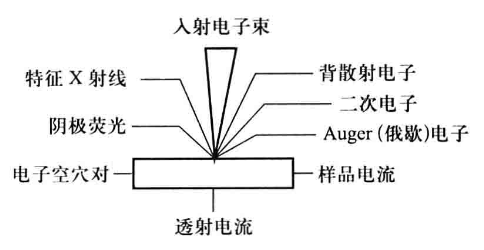
\includegraphics[width=0.4\textwidth]{fig/signal.png}
  \caption{电子入射样品产生的主要信号种类}
  \label{fig:signal}
\end{figure}
\section{实验内容}
本次实验使用SEM探测金属小球的二次电子信号,并对其进行成像。使用SEM进行成像的基本步骤如下:
\begin{enumerate}
  \item 将样品放入SEM的样品室中,并且进行抽真空。在系统进入高真空状态之后,打开电子束。
  \item 调节样品台的位置,并且调整仪器的亮度和对比度(软件提供了自动调节亮度对比度的程序,也可以手动对这两个参数进行调节),使得能够在观察屏幕上看到样品,并且亮度适中。
  \item 选取合适的放大倍数,反复调节焦距、电子束准直和像差校正,使得能够清晰的在观察屏幕上看到样品的表面形貌。
  \item 点击截屏选项,保存图像。
\end{enumerate}

随后,我们改变加速电压和束斑直径,在每一个参数组合下,对锌小球进行5000倍和20000倍的成像。最后,我们通过对金粒的成像,确定SEM的分辨极限。
\section{实验结果与分析}
\subsection{SEM成像}
实验得到的20000倍和5000倍的SEM成像如\autoref{fig:sem_photos1} 和\autoref{fig:sem_photos2} 所示。可以发现,不论是哪个放大倍数,相同的束斑直径下,加速电压越高,成像的清晰度越高。这是因为高能电子束与样品相互作用时,可以激发出更多的二次电子,从而增强信号强度,提高图像的亮度和对比度。同时,在高加速电压下,电子束在样品中的散射角度较小,会导致分辨率的提高。但是这里要说明的是,我们的加速电压最高只取道30 keV,如果继续增加加速电压,可能会导致成像的质量下降,这是因为过高的电压下电子束的穿透力过强,使得表面细节的对比度减弱。

同时我们可以发现在相同的加速电压下,不同的束斑直径成像效果也是不同的。束斑直径指的是电子束在样品表面聚焦的直径,可以通过调整系统的会聚镜和物镜,选择不同大小的孔径光阑来实现。理论上,束斑直径越小,电子束越细,在样品表面扫描时分辨率越高,但是实际上,过小的束斑直径会导致激发的二次电子数量减少,从而使得图像的亮度和对比度下降。因此,我们需要在分辨率和对比度之间进行权衡,选择合适的束斑直径。从\autoref{fig:sem_photos1} 和\autoref{fig:sem_photos2} 中总体看来,束斑直径为3.0的成像效果是最好的,这是因为在这个束斑直径下,分辨率和对比度都能够得到较好的平衡。
\begin{figure}
  \centering
  \subfigure[HV=30.0 kV, spot size=5.0]{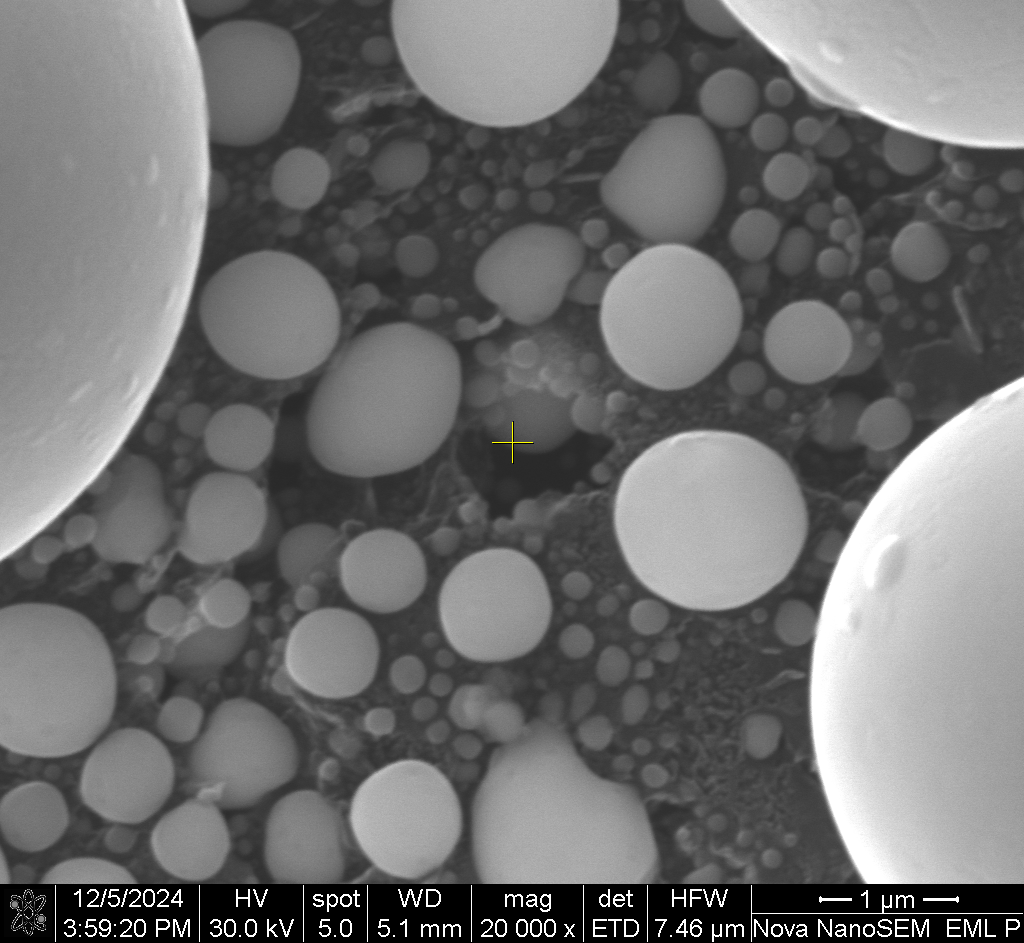
\includegraphics[height=0.3\textwidth]{fig/sem_photos/30 kV-5.0_20000x SE.png}}
  \subfigure[HV=30.0 kV, spot size=3.0]{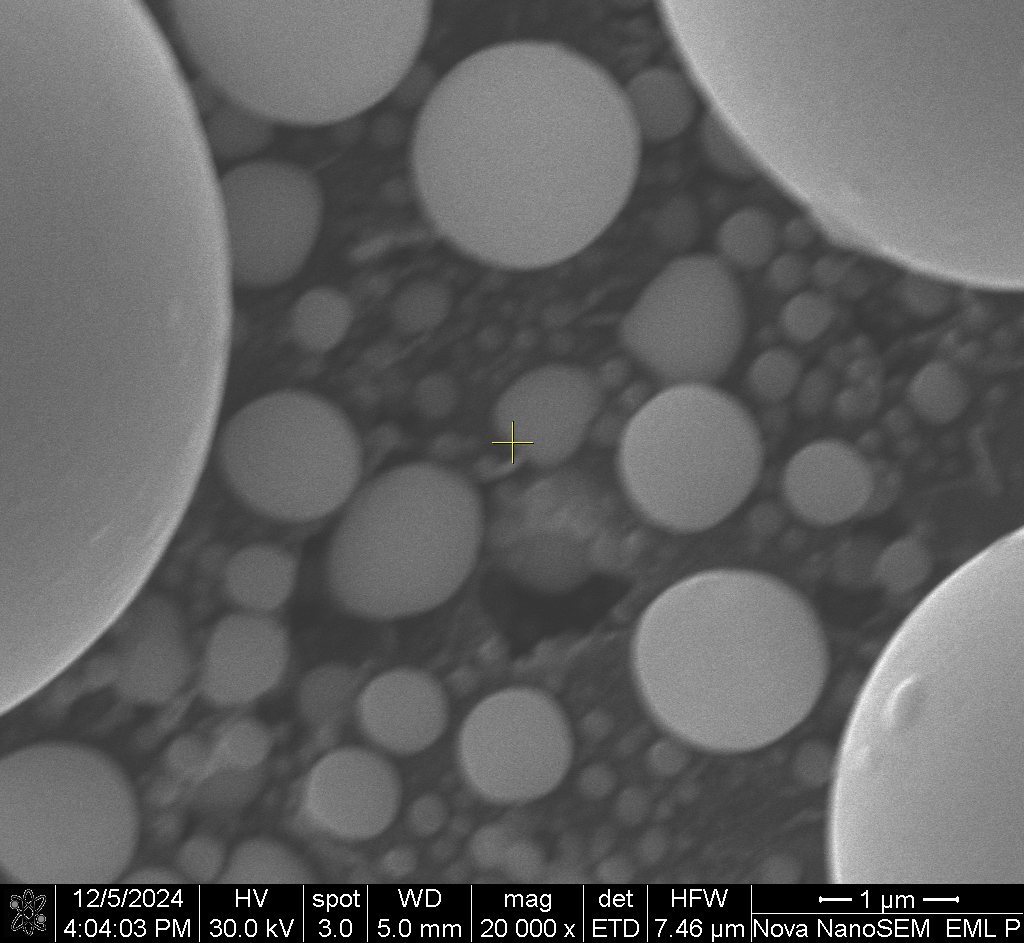
\includegraphics[height=0.3\textwidth]{fig/sem_photos/30 kV-3.0_20000x SE.png}}
  \subfigure[HV=30.0 kV, spot size=2.0]{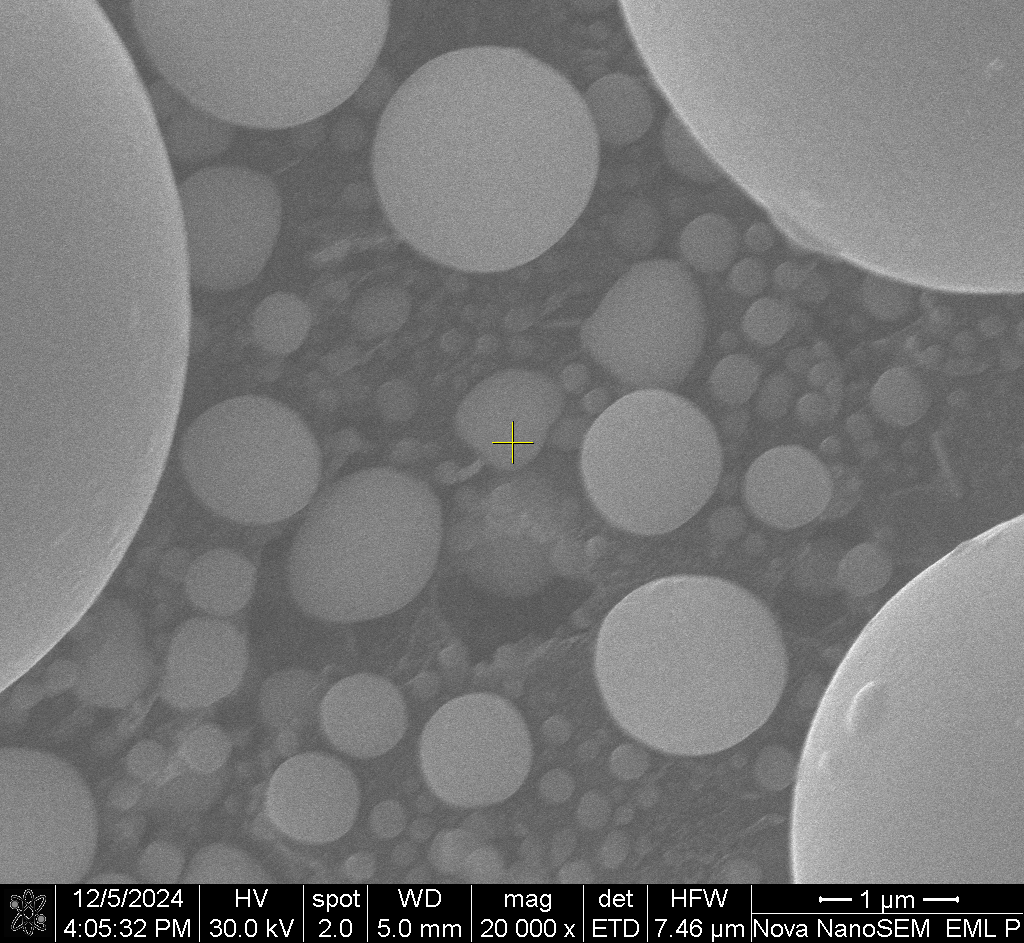
\includegraphics[height=0.3\textwidth]{fig/sem_photos/30 kV-2.0_20000x SE.png}}
  \subfigure[HV=15.0 kV, spot size=5.0]{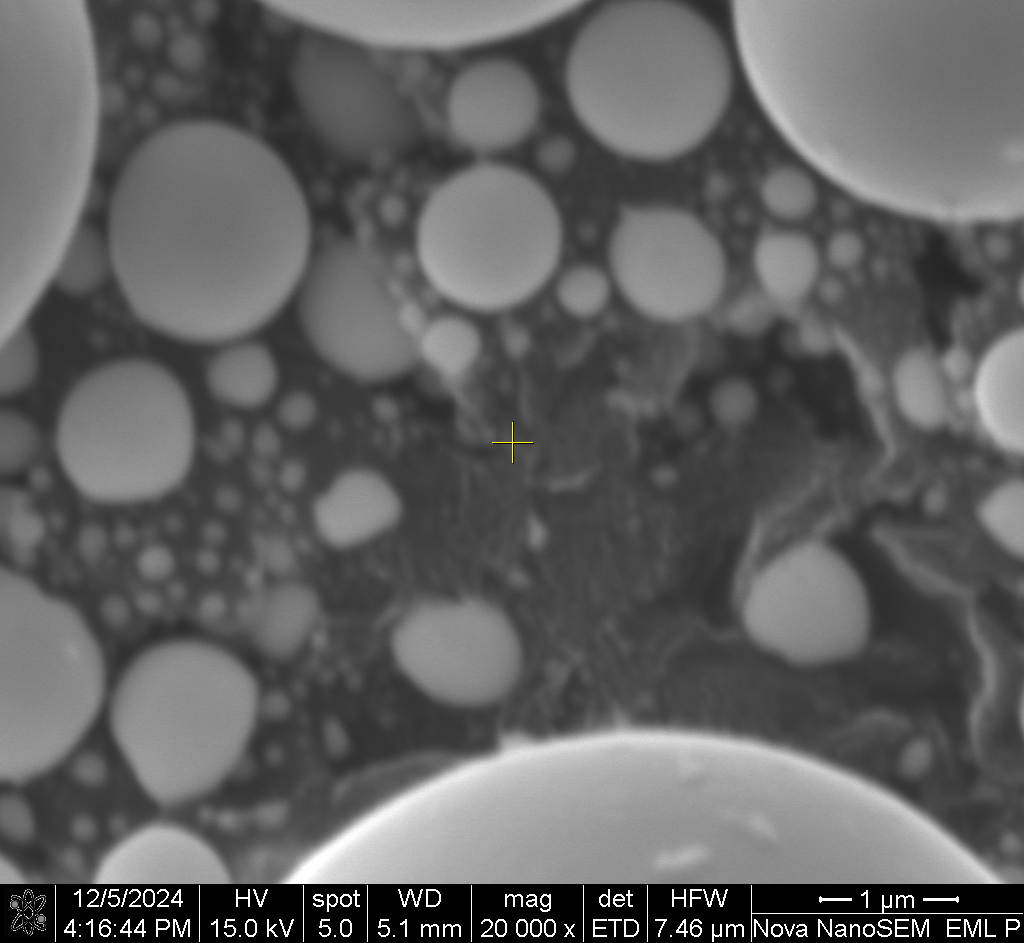
\includegraphics[height=0.3\textwidth]{fig/sem_photos/15 kV-5.0_20000x SE.png}}
  \subfigure[HV=15.0 kV, spot size=3.0]{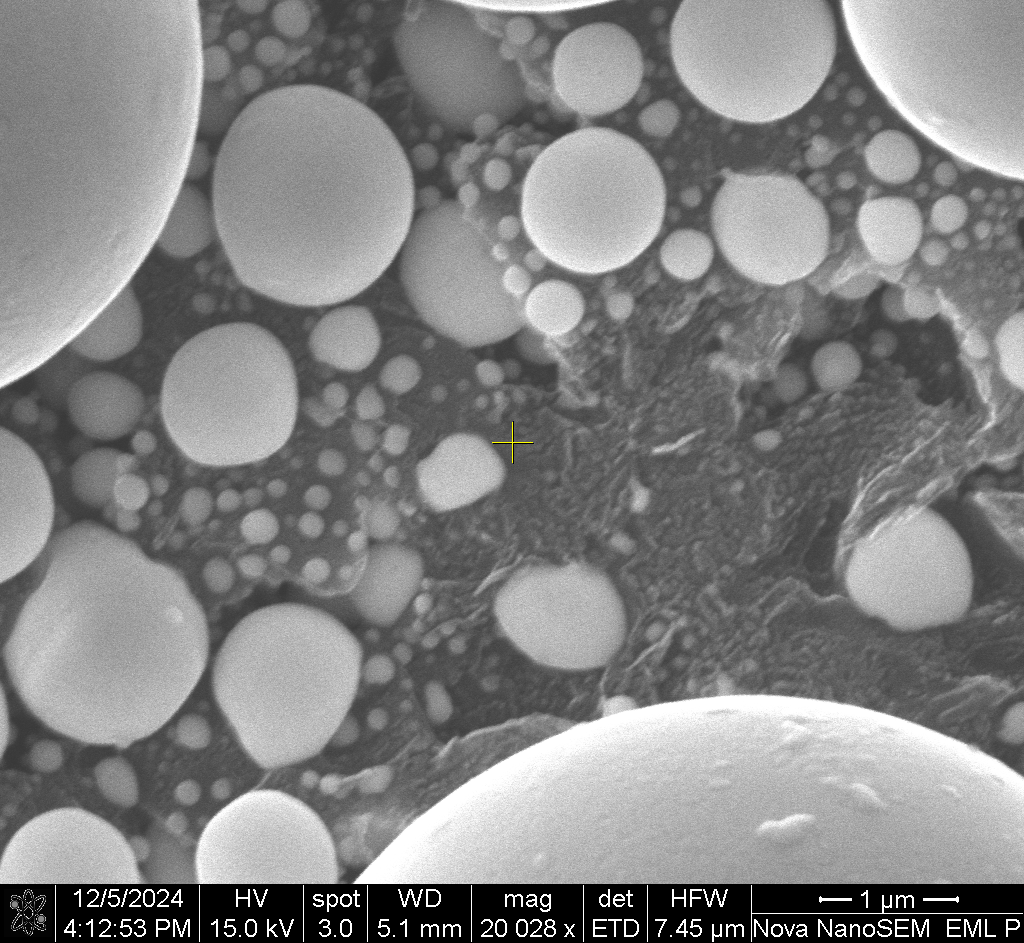
\includegraphics[height=0.3\textwidth]{fig/sem_photos/15 kV-3.0_20000x SE.png}}
  \subfigure[HV=15.0 kV, spot size=2.0]{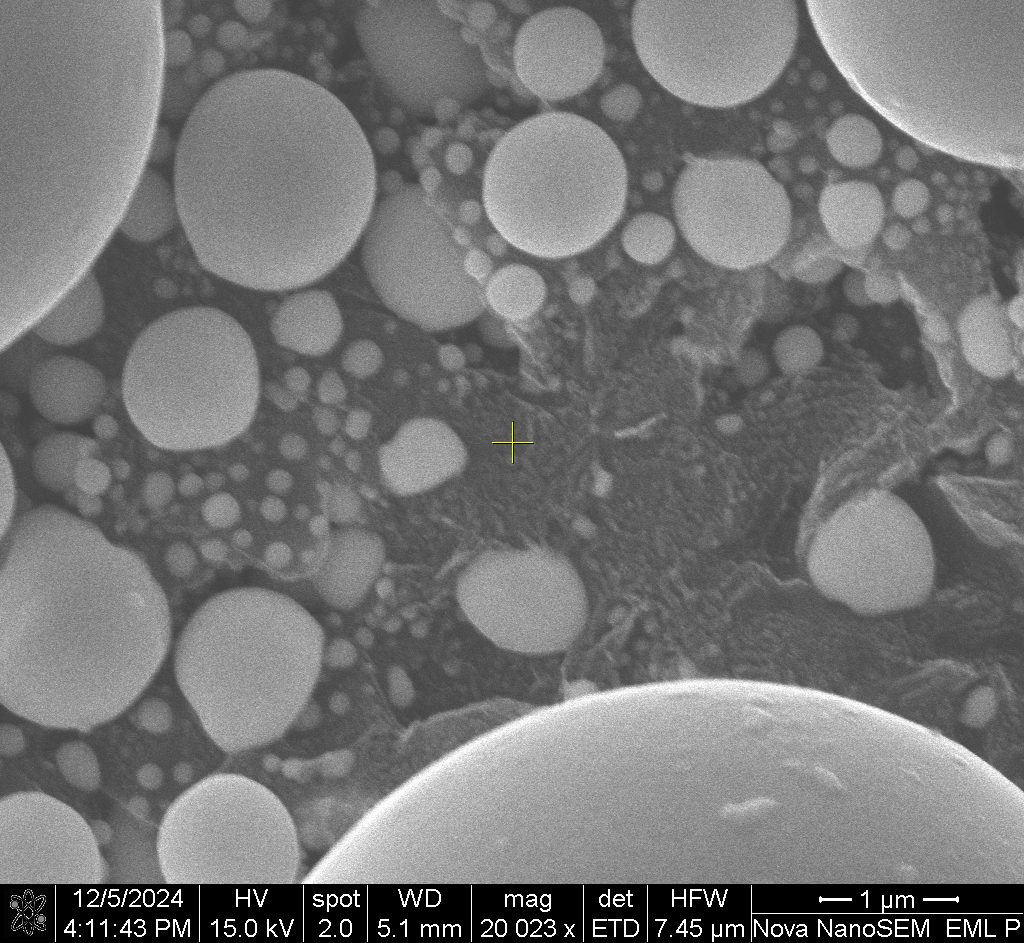
\includegraphics[height=0.3\textwidth]{fig/sem_photos/15 kV-2.0_20000x SE.png}}
  \subfigure[HV=2.0 kV, spot size=5.0]{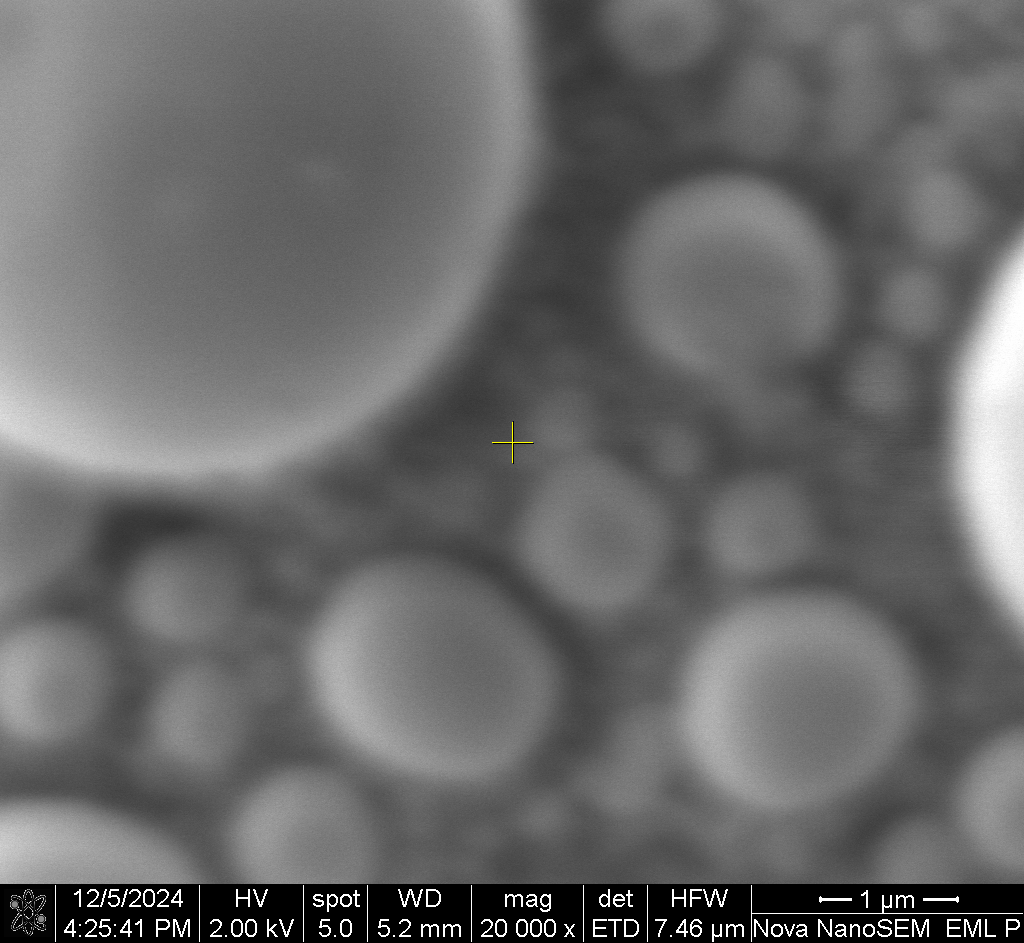
\includegraphics[height=0.3\textwidth]{fig/sem_photos/2 kV-5.0_20000x SE.png}}
  \subfigure[HV=2.0 kV, spot size=3.0]{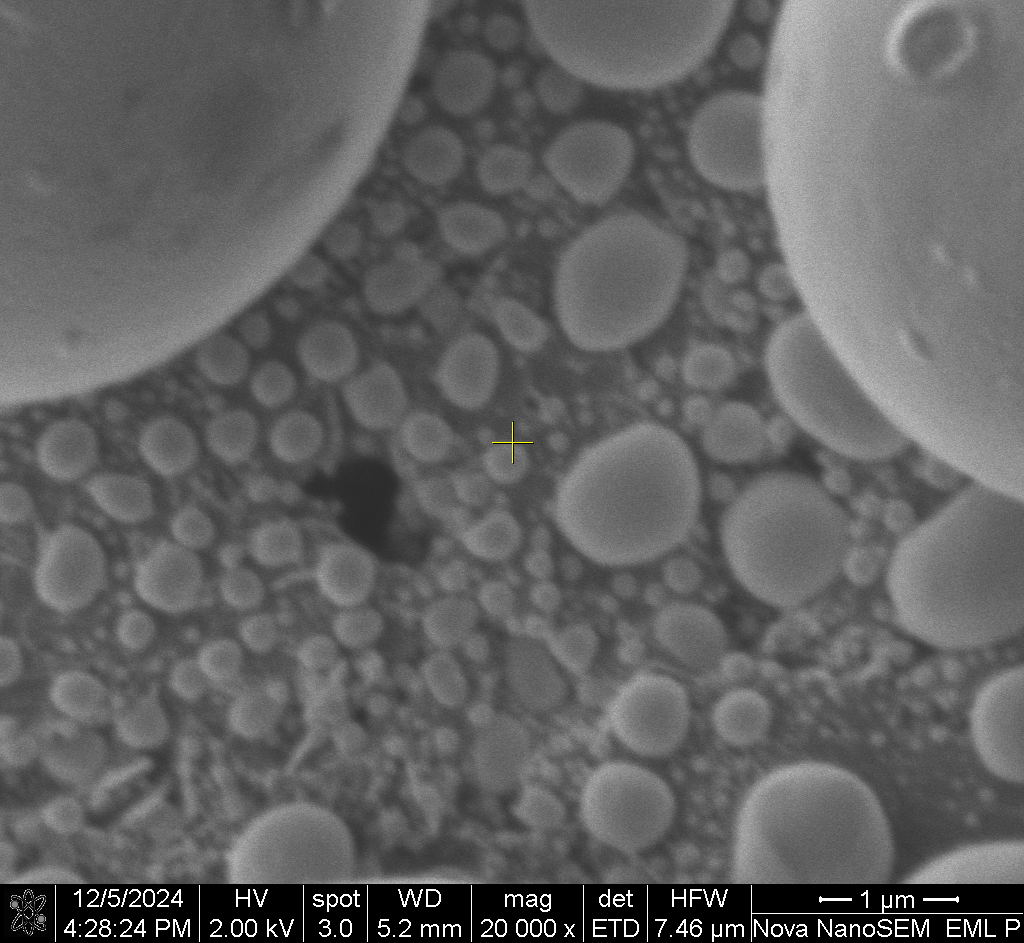
\includegraphics[height=0.3\textwidth]{fig/sem_photos/2 kV-3.0_20000x SE.png}}
  \subfigure[HV=2.0 kV, spot size=2.0]{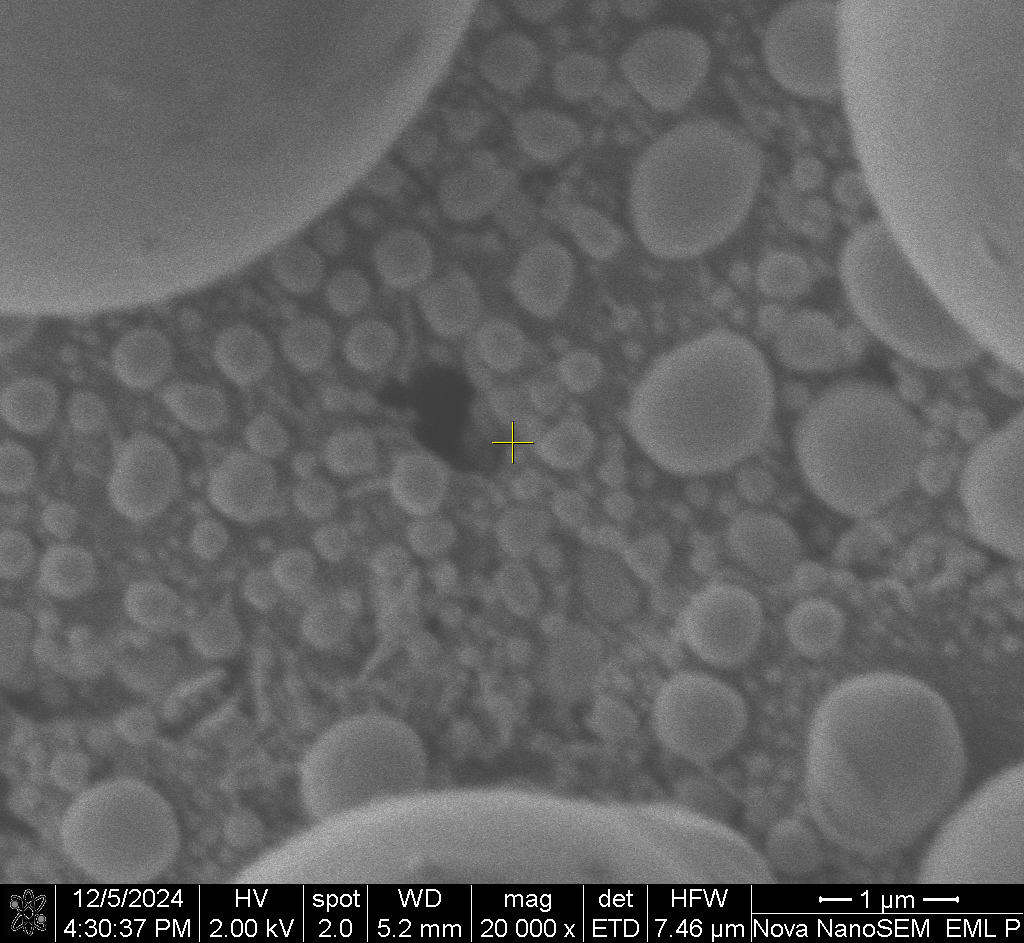
\includegraphics[height=0.3\textwidth]{fig/sem_photos/2 kV-2.0_20000x SE.png}}
  \caption{金属小球在不同的HV\footnote{HV, High Voltage,代表的是电子束的加速电压,它直接决定了电子束的动能大小。加速电压越高,电子束获得的动能越大,电子的速度也越快。}和spot size\footnote{Spot size,也称为束斑直径、探针尺寸。spot size越小,电子束越细,在样品表面扫描时分辨率越高,但激发的二次电子越少。}中的20,000倍扫描电镜成像}
  \label{fig:sem_photos1}
\end{figure}

\begin{figure}
  \centering
  \subfigure[HV=30.0 kV, spot size=5.0]{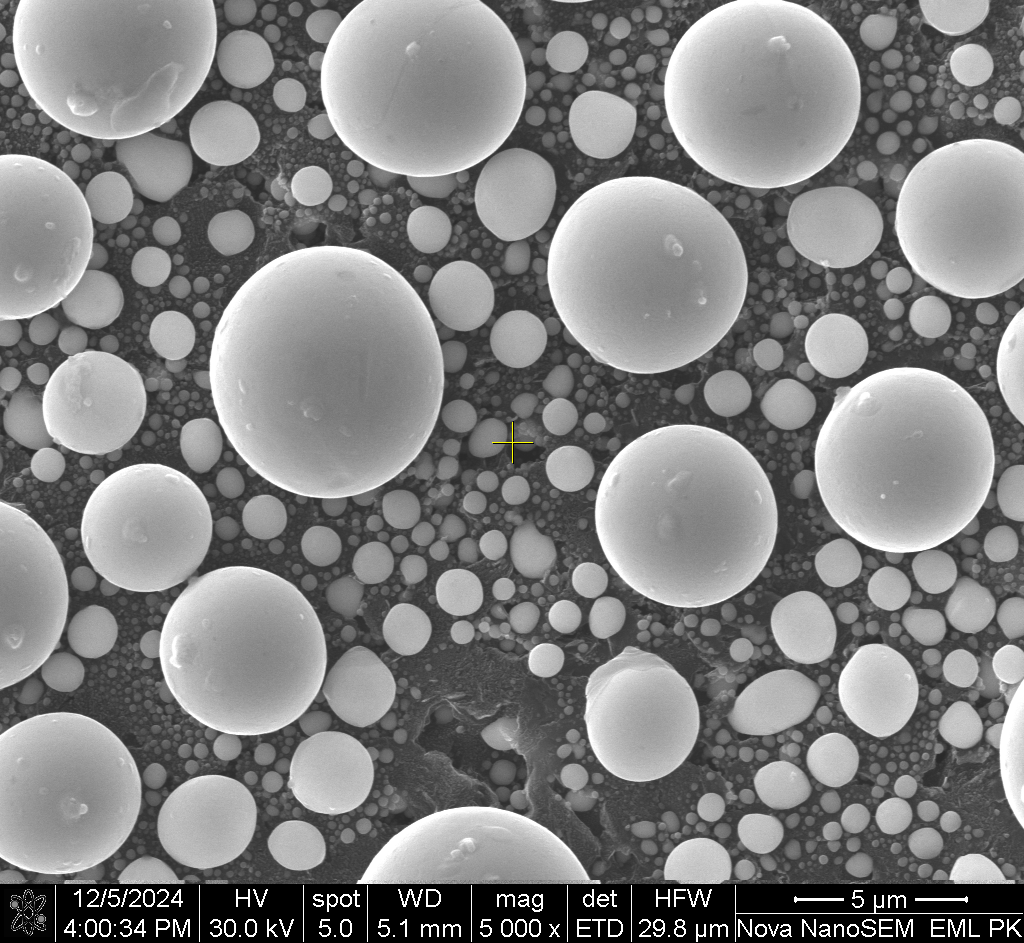
\includegraphics[height=0.3\textwidth]{fig/sem_photos/30 kV-5.0_5000x SE.png}}
  \subfigure[HV=30.0 kV, spot size=3.0]{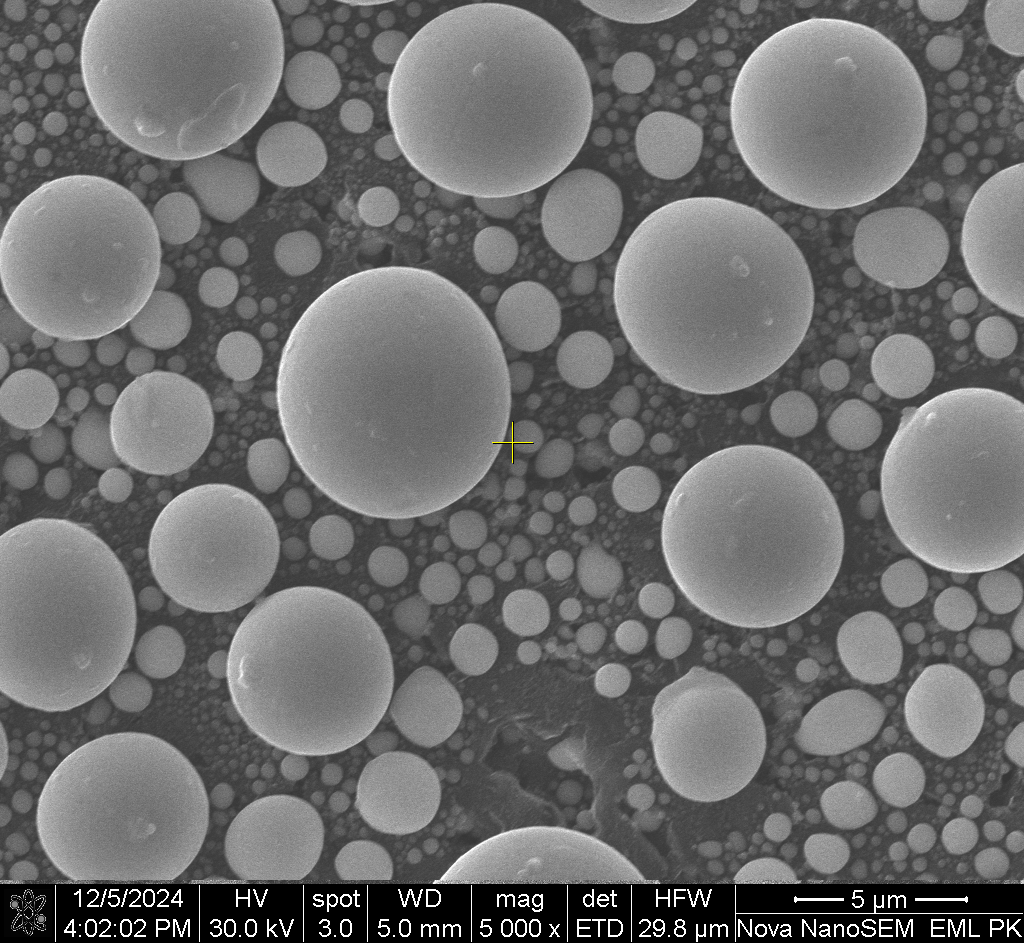
\includegraphics[height=0.3\textwidth]{fig/sem_photos/30 kV-3.0_5000x SE.png}}
  \subfigure[HV=30.0 kV, spot size=2.0]{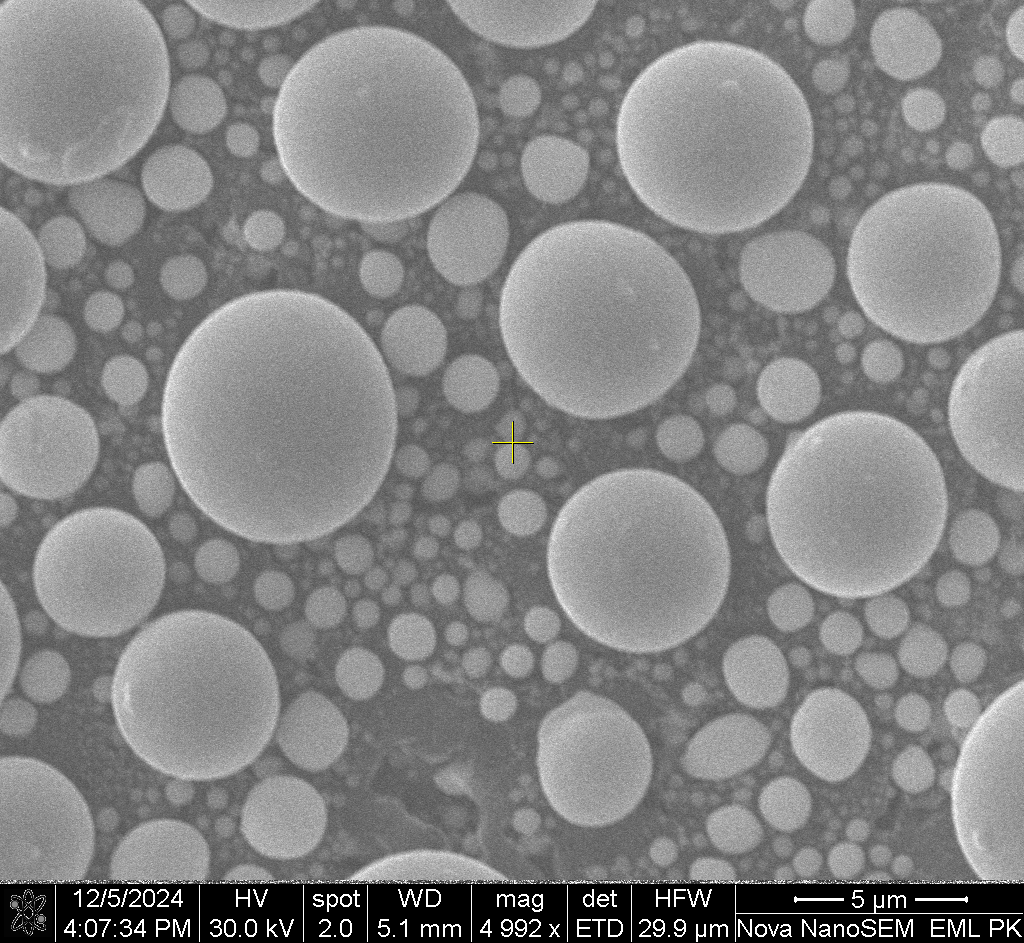
\includegraphics[height=0.3\textwidth]{fig/sem_photos/30 kV-2.0_5000x SE.png}}
  \subfigure[HV=15.0 kV, spot size=5.0]{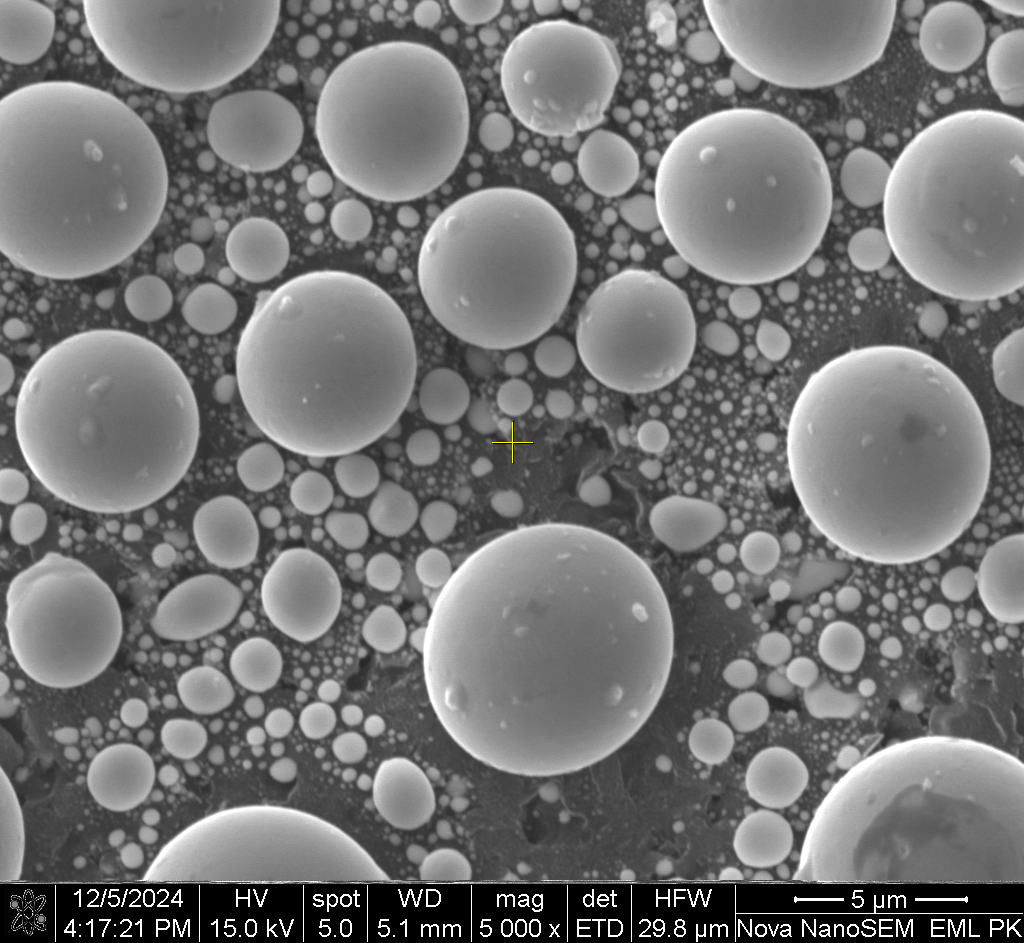
\includegraphics[height=0.3\textwidth]{fig/sem_photos/15 kV-5.0_5000x SE.png}}
  \subfigure[HV=15.0 kV, spot size=3.0]{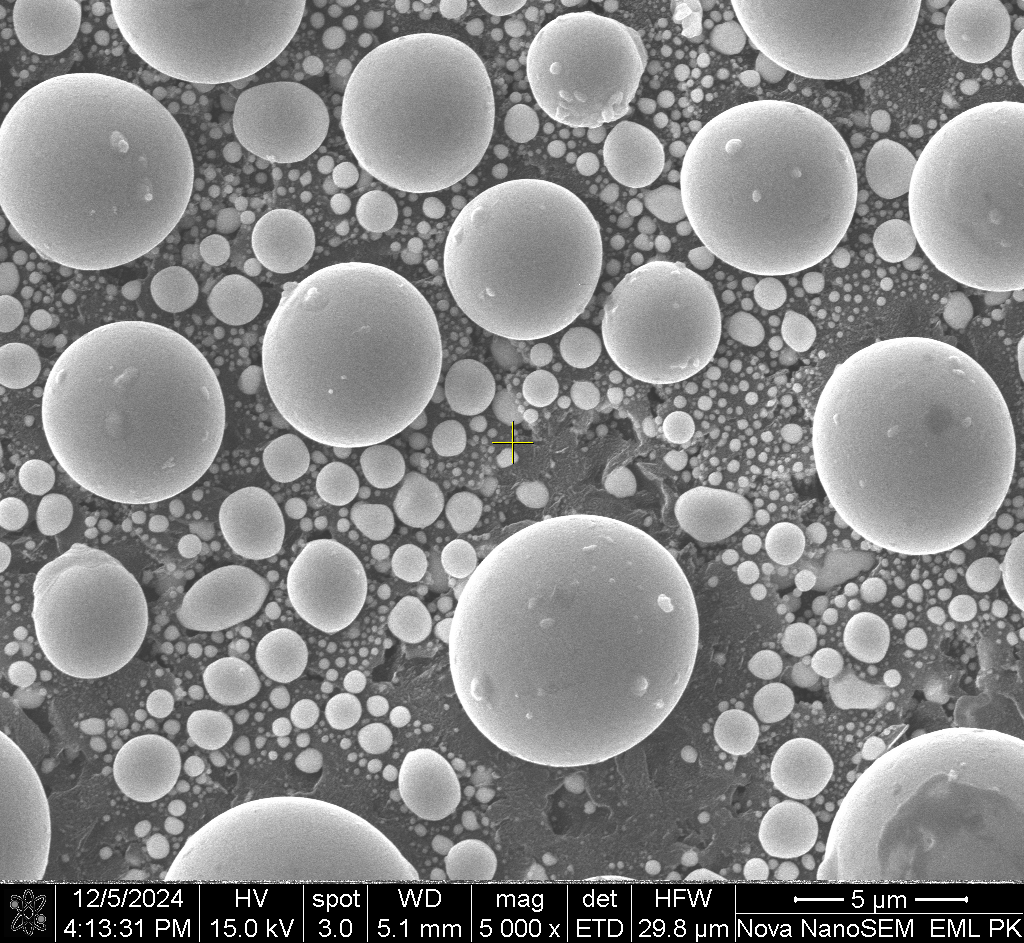
\includegraphics[height=0.3\textwidth]{fig/sem_photos/15 kV-3.0_5000x SE.png}}
  \subfigure[HV=15.0 kV, spot size=2.0]{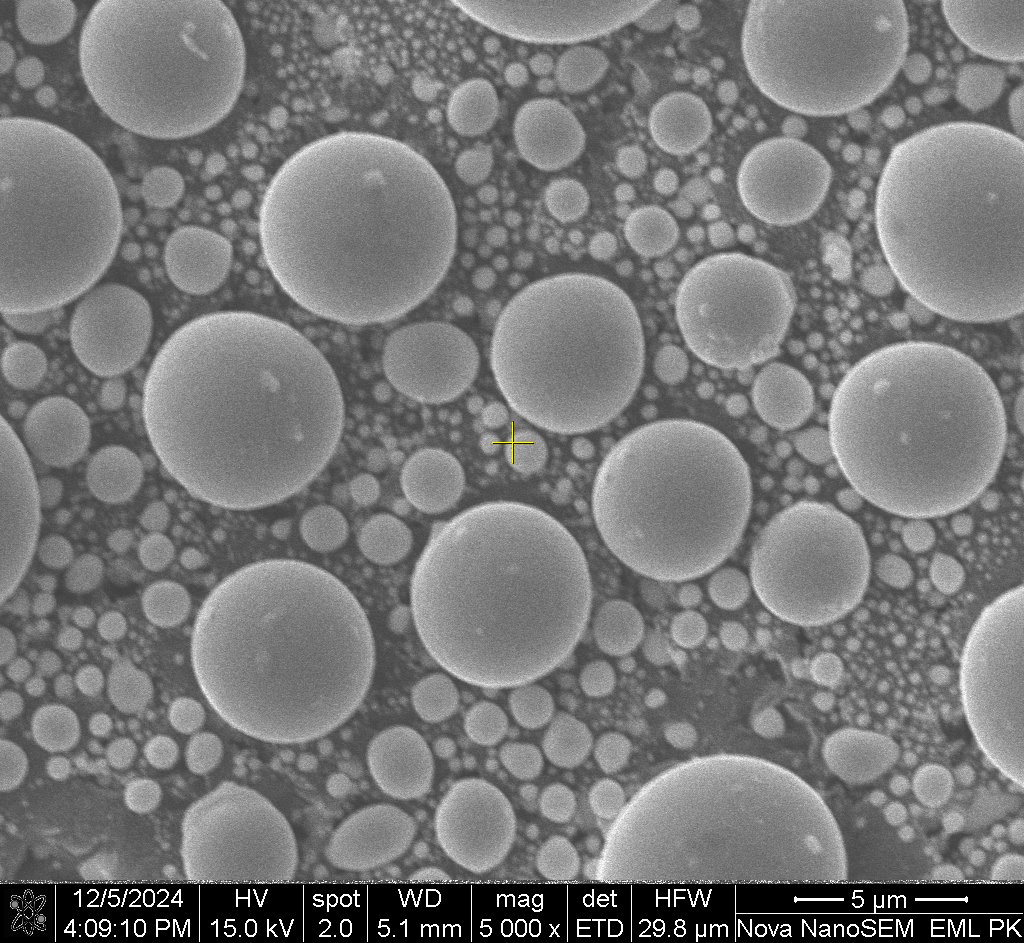
\includegraphics[height=0.3\textwidth]{fig/sem_photos/15 kV-2.0_5000x SE.png}}
  \subfigure[HV=2.0 kV, spot size=5.0]{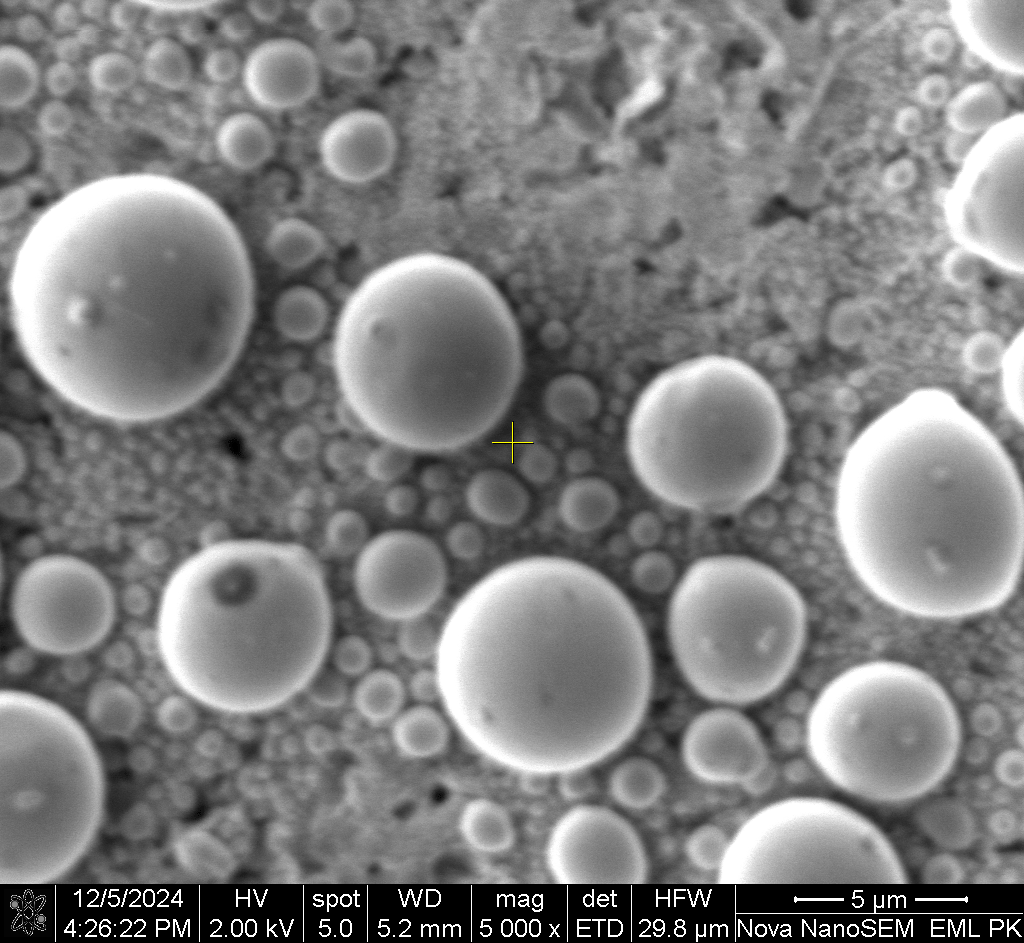
\includegraphics[height=0.3\textwidth]{fig/sem_photos/2 kV-5.0_5000x SE.png}}
  \subfigure[HV=2.0 kV, spot size=3.0]{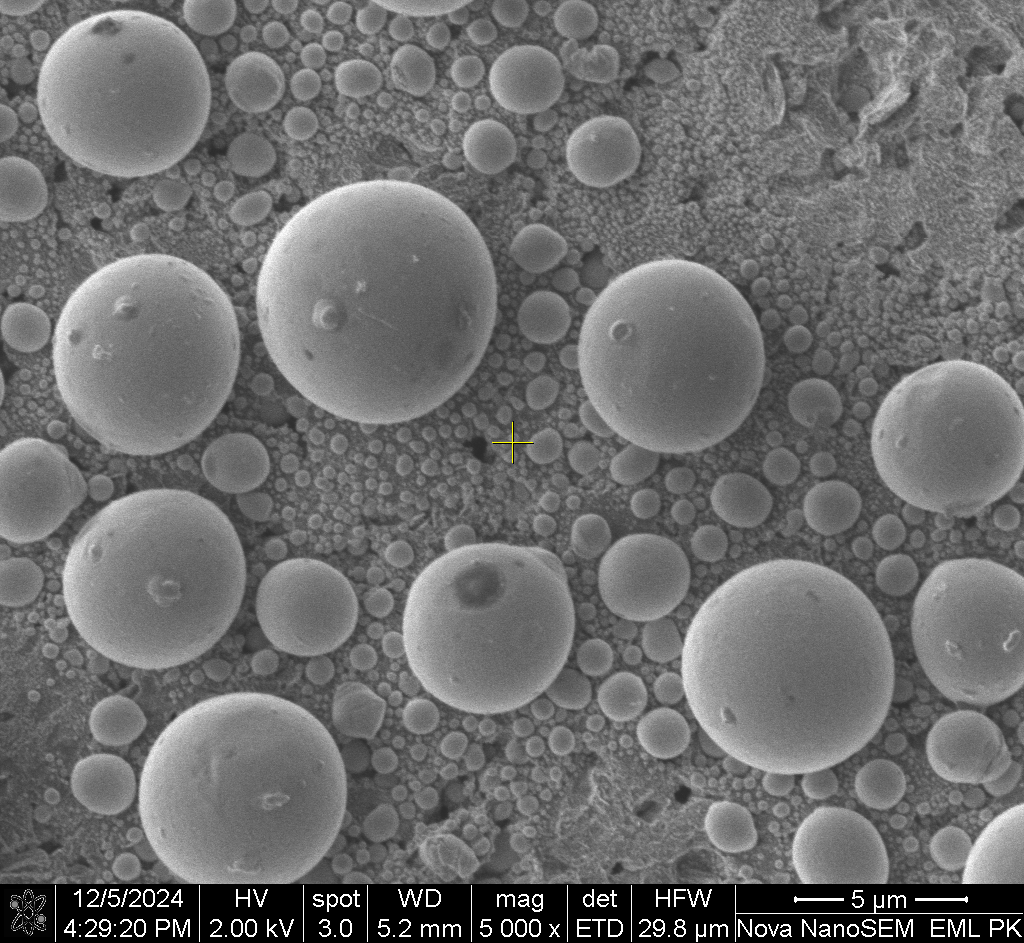
\includegraphics[height=0.3\textwidth]{fig/sem_photos/2 kV-3.0_5000x SE.png}}
  \subfigure[HV=2.0 kV, spot size=2.0]{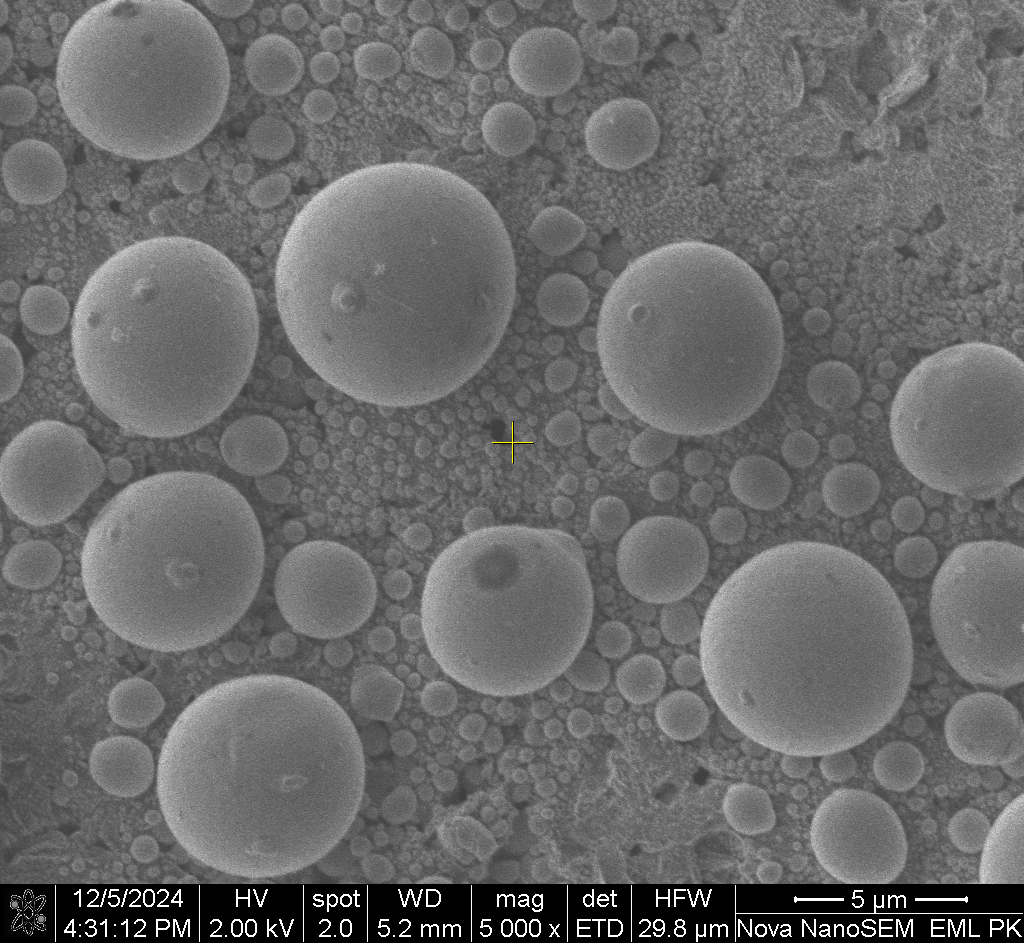
\includegraphics[height=0.3\textwidth]{fig/sem_photos/2 kV-2.0_5000x SE.png}}
  \caption{金属小球在不同的HV和spot size中的5,000倍扫描电镜成像}
  \label{fig:sem_photos2}
\end{figure}

\subsection{分辨极限}
\autoref{fig:gold} 是我们在30.0 kV的加速电压,3.0的束斑直径下拍摄的金粒的SEM图像。图中已经给出100 nm的标尺,因此我们只需要估算出图像中能够分辨的最小特征尺寸,就能够确定SEM的分辨极限。图中我们已经用红色小圈圈出能够分辨的最小金球,于是我们得到SEM的分辨极限为
\begin{equation}
  d_{\min}\approx 10\text{ nm}.
\end{equation}
\begin{figure}
  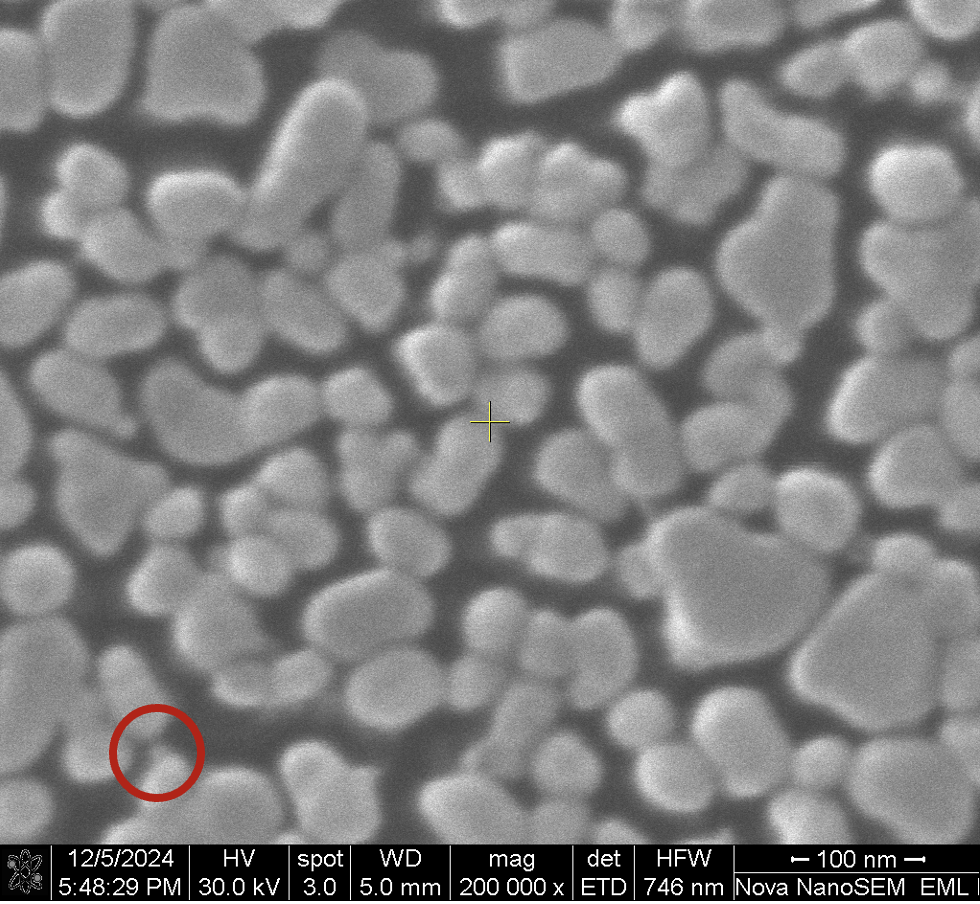
\includegraphics[height=0.3\textwidth]{fig/sem_photos/30 kV-3.0_150000x SE_fenbian_002.png}
  \caption{金粒在200,000倍扫描电镜成像。成像参数:HV=30.0 kV, spot size=3.0}
  \label{fig:gold}
\end{figure}
\section{结论}
通过本次实验,我们学会了SEM的基本使用方法,掌握了SEM的成像原理,了解了SEM的分辨极限。我们对加速电压和束斑直径两个参数进行了调节以研究它们对于成像质量的影响。在我们的研究参数范围内,我们发现30.0 kV的加速电压和3.0的束斑直径成像效果是最好的。此外,我们还对上面的结果做出了简要分析。最后,我们通过对金粒的成像,确定了SEM的分辨极限为 10 nm。

\appendix

\section{思考题}
\subsection{如何确定照片上图像的放大倍数?}
一般来说,SEM的图像上会有放大倍数这个参数,这是能够最直接确定图像放大倍数的方法。例如图像上显示的mag 20 000 x就表示放大倍数为20000倍。此外,我们还可以通过SEM图像中的标尺来确定放大倍数:通过测量图像中某个已知尺寸的特征,并与标尺上的长度进行比较,可以计算出放大倍数。

若SEM图像上没有显示上面任意之一的参数,那么我们就要通过估算的方法。首先,我们应该估算图像中的样品的实际尺寸,然后通过测量图像中的样品尺寸确定放大倍数。这依赖于我们对于测量样品的先验知识。
\subsection{如何评价一幅SEM照片的优劣?}
首先SEM照片需要有高分辨率,能够清晰地显示样品的细节和显微结构,信噪比足够大,衬度适中,能够突出样品的特征。其次对于具有一定厚度分布的样品,成像的景深要足够大,需要使整个样品都能清晰成像,而不仅仅是表面。最后,图像应能准确地代表样品的整体特征,不是局部或异常的表现。

\end{document}
